\section{割近似与谱近似}
\label{sec:graph-sparsification-approximation}

稀疏化的目标是用一张边少得多的图来代替原图。但代替到什么程度才算够用？本节先从割权开始回答这个问题，再把要求提高到所有实值向量上的能量。

\subsection{割近似}
\label{sec:graph-cut-approximation}

假设原来某个割的权是十。如果允许百分之十的误差，替代图上这个割的权落在九和十一之间就算可以接受。如果原来的割权为零，相对误差要求替代图上也是零——两团之间没边的判断不能弄错。

但是，稀疏化是在看到任何特定的割之前就已经选定了一张替代图。之后在替代图上搜索最小割时，算法会逐一比较各种分组，其中可能恰好有一种分组的跨边被删掉了许多。因此我们要求先固定替代图，再让它对\emph{每一个}分组都满足同一个相对误差。

\begin{definition}[割近似]
\label{def:graph-cut-approximation}
设$\mathcal G$与$\mathcal H$有同一顶点集$V$，$0<\varepsilon<1$。对$S\subseteq V$，记$\overline S=V\setminus S$，用$c_G(S,\overline S)$和$c_H(S,\overline S)$分别表示两图中跨越该割的边权之和。若每个$S$都满足
\begin{equation}
(1-\varepsilon)c_G(S,\overline S)
\leq c_H(S,\overline S)
\leq (1+\varepsilon)c_G(S,\overline S),
\label{eq:graph-cut-approximation}
\end{equation}
就说$\mathcal H$是$\mathcal G$的一个$\varepsilon$\term{割近似}（cut approximation）。
\end{definition}

下界系数$1-\varepsilon$是正数，所以原图中有正权边跨越的割，在$\mathcal H$中仍有正权边跨越。零割也自动保持为零。这保证了"某一组顶点与外部是否相连"的判断不变。

\paragraph{最小割的继承}

记$C_G$和$C_H$为两图的最小割权。两图的分组候选完全相同，但取到最小值的分组可能不同。

先给$C_H$找一个下界。设$S^*_H$是$\mathcal H$中的最优分组，按割近似的上界，它在$\mathcal H$中的割权至多是它在$\mathcal G$中割权的$1+\varepsilon$倍。反过来，$\mathcal G$中的最优分组$S^*_G$作为$\mathcal H$的一个候选，其在$\mathcal H$中的割权至少是在$\mathcal G$中的$1-\varepsilon$倍。$\mathcal H$的最小割不超过任何候选，$\mathcal G$的最小割不超过$S^*_H$在$\mathcal G$上的值，因此
\begin{equation}
(1-\varepsilon)C_G\leq C_H\leq(1+\varepsilon)C_G.
\label{eq:graph-sparsification-min-cut}
\end{equation}

\paragraph{RatioCut的继承}

第~\ref{chap:spectral-partition}章的RatioCut把割权乘以$1/|S|+1/|\overline S|$。两图共享同一个顶点集，因此这个因子在每个割上完全相同。割权的$1\pm\varepsilon$比例直接传给了RatioCut的目标值，最优值也是如此。

\paragraph{体积和导通率的继承}

导通率和NCut还用到集合的\emph{体积}，即一侧顶点的加权度之和$\operatorname{vol}_G(S)=\sum_{i\in S}d_i$。换了边权后，各顶点的加权度也会改变。

取单点集合$\{v\}$。它的割恰好由$v$的所有关联边组成，因此式~\eqref{eq:graph-cut-approximation}也控制了每个顶点的加权度。将组内所有顶点的度下界相加或上界相加，得到
\begin{equation}
(1-\varepsilon)\operatorname{vol}_G(S)
\leq \operatorname{vol}_H(S)
\leq (1+\varepsilon)\operatorname{vol}_G(S).
\label{eq:graph-sparsification-volume}
\end{equation}
需要注意的是，组内边在组内两个顶点的度里各计一次，但在$S$的割权中不出现。

第~\ref{sec:graph-cheeger}节的导通率以割权为分子、以较小一侧的体积为分母。分子和分母都可能偏离原值。用割权下界除以体积上界，可以得到导通率的下界；用割权上界除以体积下界，得到上界。记两图的导通率为$\phi_G(S)$和$\phi_H(S)$，整理后
\begin{equation}
\frac{1-\varepsilon}{1+\varepsilon}\phi_G(S)
\leq \phi_H(S)
\leq \frac{1+\varepsilon}{1-\varepsilon}\phi_G(S).
\label{eq:graph-sparsification-conductance}
\end{equation}
NCut是割权分别除以两侧体积之后的和。每一项都继承同样的比例界，两图的正体积集合相同，因此可以在相同的合法划分上取最小来比较最优值。

\subsection{谱近似}
\label{sec:graph-spectral-approximation}

割近似只看指示向量——每个顶点要么在$S$中取一、要么在$\overline S$中取零。这时跨割边两端的差平方都是一，能量就等于跨割的边权之和。

但谱划分的松弛和拉普拉斯方程用到的是\emph{任意实值}的顶点赋值。两端相差五的那条边和两端相差零点一的那条边，对能量的贡献可以差几个数量级。单纯比较跨边总权看不出重加权集中在差异大的边还是差异小的边。因此需要一种更严格的保证：让替代图在\emph{每一种}赋值上的能量都接近原图。

\begin{definition}[谱近似]
\label{def:graph-spectral-approximation}
设$\bm L_G$和$\bm L_H$是同一顶点集上两图的拉普拉斯矩阵。若对每个$\bm x\in\mathbb R^n$都有
\begin{equation}
(1-\varepsilon)\bm x^\top\bm L_G\bm x
\leq \bm x^\top\bm L_H\bm x
\leq (1+\varepsilon)\bm x^\top\bm L_G\bm x,
\label{eq:graph-spectral-approximation-energy}
\end{equation}
则称$\mathcal H$是$\mathcal G$的一个$\varepsilon$\term{谱近似}（spectral approximation）。用半正定序写，就是
\begin{equation}
(1-\varepsilon)\bm L_G\preceq\bm L_H\preceq(1+\varepsilon)\bm L_G.
\label{eq:graph-spectral-approximation-order}
\end{equation}
边数显著减少且满足此条件的构造称为\term{谱稀疏化}（spectral sparsification）。
\end{definition}

谱近似蕴含割近似。只需在式~\eqref{eq:graph-spectral-approximation-energy}中把$\bm x$取成子集$S$的指示向量——只有跨割边的两端值不同，差的平方都是一，因此能量恰好等于割权。代入后就得到式~\eqref{eq:graph-cut-approximation}。

谱近似还自动保留连通分量。若$\bm x^\top\bm L_G\bm x=0$，上界迫使$\bm x^\top\bm L_H\bm x=0$。反过来，若$\bm x^\top\bm L_H\bm x=0$，正的下界系数$1-\varepsilon$迫使原图能量也为零。第~\ref{sec:graph-laplacian-kernel}节说过，能量为零要求在每个正权连通分量上取常值。因此两图的零能量方向完全相同，连通分量也完全相同。

对连通图，只有常值方向的能量为零。在$\bm 1^\perp$中，非零向量的能量为正，可以取拉普拉斯的逆。

\paragraph{割近似不蕴含谱近似}

反过来的推论不成立。下面用一个三顶点的例子说明，满足割近似的替代图在某个实值向量上的能量可以超出谱近似的允许范围。

\begin{example}[满足割界的图可以超出同一谱界]
\label{ex:graph-cut-not-spectral}
令$\mathcal G$是单位权三角形，三条边的权都是一。取$0<\varepsilon<1/2$，构造替代图$\mathcal H$：把边$12$的权增加$2\varepsilon$，把边$23$的权减少$2\varepsilon$，边$13$保持不变，
\[
c_H(12)=1+2\varepsilon,\qquad c_H(23)=1-2\varepsilon,\qquad c_H(13)=1.
\]

先检查割近似。原图中每个顶点都连着两条单位权边，三个单点割的权都是二。替代图中：顶点$1$的两条边权之和为$(1+2\varepsilon)+1=2+2\varepsilon$，顶点$2$的为$(1+2\varepsilon)+(1-2\varepsilon)=2$，顶点$3$的为$(1-2\varepsilon)+1=2-2\varepsilon$。三个数都落在$2(1\pm\varepsilon)$之间。因为两点割和它的单点补割权相同，所以全部六个非平凡割都满足式~\eqref{eq:graph-cut-approximation}。

再取顶点赋值$\bm x=(3,-2,-1)^\top$。三条边上两端差的平方分别是
\[
(3-(-2))^2=25,\qquad ((-2)-(-1))^2=1,\qquad (3-(-1))^2=16.
\]
原图能量为$25+1+16=42$。替代图的能量为
\[
25(1+2\varepsilon)+1\cdot(1-2\varepsilon)+16\cdot1=42+48\varepsilon.
\]
比如取$\varepsilon=1/4$。此时所有割权都在原值的$75\%$到$125\%$之间——割近似完全满足。但这个向量的能量从$42$升到了$54$，超过了谱近似允许的上界$42\times 5/4=52.5$。

能量比为$1+48\varepsilon/42=1+8\varepsilon/7$，严格大于$1+\varepsilon$。原因在于：顶点$2$的单点割看到的两条边权一增一减，总和不变。但这个实值赋值在边$12$上的差平方为$25$，在边$23$上只有$1$，增权集中在能量高的边上，减权集中在能量低的边上，二者无法对消。图~\ref{fig:sparsification-cut-energy}并排画出两图和同一个赋值，便于逐边比较。
\end{example}

\begin{BookInlineFigure}
  \centering
  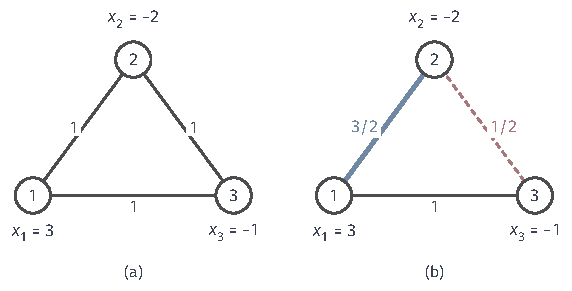
\includegraphics{figures/03-graphs/05-matrices-and-spectra/tikz/sparsification-cut-energy/figure.pdf}
  \caption{单位权原图（a）和取$\varepsilon=1/4$的替代图（b）。粗实线表示增重的边，虚线表示减重的边。三个单点割的权都满足$1\pm\varepsilon$比例，但按相同的顶点赋值$(3,-2,-1)$计算能量，替代图从$42$升到$54$，超出了谱近似的允许范围。}
  \label{fig:sparsification-cut-energy}
\end{BookInlineFigure}


\subsection{谱近似保持的量}
\label{sec:graph-spectral-approximation-consequences}

有了谱近似图，可以用它来估计原图的特征值、有效电阻和方程解。这三种比较共用同一个能量界，但各自控制的量不同：特征值来自能量商的极值，后两种还需要把比较从拉普拉斯传到逆矩阵上。

\paragraph{特征值的保持}

先把两图的组合拉普拉斯特征值各按从小到大排序。对每个$i$，想要比较第$i$个特征值。

式~\eqref{eq:graph-spectral-approximation-energy}对每个非零向量成立，两边同除以$\bm x^\top\bm x$仍然成立。左边和右边变成了Rayleigh商的比例界。在同一个$i$维子空间上分别对两图取商的最大值，原来的比例界不变。再在所有$i$维子空间中取最小值——Courant--Fischer原理（可参考\BookChapterRef{chap:condition-and-spectral-perturbation}{卷二"条件数与谱扰动"章}）说这个极值就是第$i$个特征值。因此
\begin{equation}
(1-\varepsilon)\lambda_i(\bm L_G)
\leq \lambda_i(\bm L_H)
\leq (1+\varepsilon)\lambda_i(\bm L_G).
\label{eq:graph-sparsification-eigenvalue}
\end{equation}
这只比较排序后的谱值。逐个特征向量或子空间的稳定性需要额外分析，特别是在特征值接近时。

\paragraph{有效电阻的保持}

有效电阻用到拉普拉斯的逆。为了把能量的正向比较变成逆矩阵的比较，先换一套坐标，让原图变成单位矩阵。

设原图连通，在$\bm 1^\perp$上操作。令$\bm y=\bm L_G^{1/2}\bm x$，原图能量就是$\lVert\bm y\rVert_2^2$。将$\bm x=\bm L_G^{-1/2}\bm y$代入替代图的能量，得到$\bm y^\top\bm A\bm y$，其中
\[
\bm A=\bm L_G^{-1/2}\bm L_H\bm L_G^{-1/2}.
\]
能量界对每个$\bm y$成立，因此
\begin{equation}
(1-\varepsilon)\bm I\preceq\bm A\preceq(1+\varepsilon)\bm I.
\label{eq:graph-sparsification-normalized-order}
\end{equation}
这意味着$\bm A$的每个特征值都落在$[1-\varepsilon,1+\varepsilon]$中。

取逆就是对同一组正交特征方向分别取倒数。$1-\varepsilon$变成$1/(1-\varepsilon)$，$1+\varepsilon$变成$1/(1+\varepsilon)$。注意取倒数会翻转大小关系——原来的下界变成了新的上界。图~\ref{fig:sparsification-inverse-band}用数轴标出这个翻转。

\begin{BookInlineFigure}
  \centering
  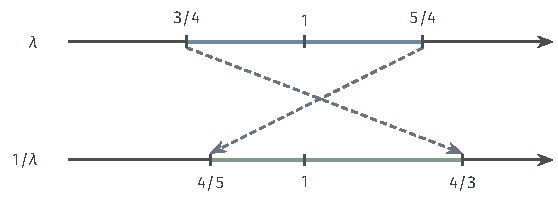
\includegraphics{figures/03-graphs/05-matrices-and-spectra/tikz/sparsification-inverse-band/figure.pdf}
  \caption{能量坐标中谱值的允许区间。虚线示意两端取倒数后怎样换位：靠左的$1-\varepsilon$变到$1/(1-\varepsilon)$一端。中间的$1$保持不动。}
  \label{fig:sparsification-inverse-band}
\end{BookInlineFigure}

将三个因子依次反向取逆，$\bm A^{-1}=\bm L_G^{1/2}\bm L_H^{-1}\bm L_G^{1/2}$。对逆矩阵的比较式两边同乘$\bm L_G^{-1/2}$，中间还原为$\bm L_H^{-1}$，上下界的单位阵还原为$\bm L_G^{-1}$。在全体向量上，两个逆都在常数方向取零，由此得到伪逆的比较
\begin{equation}
\frac{1}{1+\varepsilon}\bm L_G^\dagger
\preceq \bm L_H^\dagger
\preceq \frac{1}{1-\varepsilon}\bm L_G^\dagger.
\label{eq:graph-sparsification-inverse-order}
\end{equation}

把两点差向量$\bm e_u-\bm e_v$代入这三个二次型。按第~\ref{sec:graph-effective-resistance}节的有效电阻公式，
\begin{equation}
\frac{R_G(u,v)}{1+\varepsilon}
\leq R_H(u,v)
\leq \frac{R_G(u,v)}{1-\varepsilon}.
\label{eq:graph-sparsification-resistance}
\end{equation}
直觉上，替代图若整体提高了能量，通相同电流所需的电势差会降低——这对应了取逆之后比例关系的翻转。

\paragraph{方程解的保持}

设$\bm b\in\bm 1^\perp$，$\bm x_G=\bm L_G^\dagger\bm b$是原图的零均值解，$\bm x_H=\bm L_H^\dagger\bm b$是替代图的零均值解。我们想知道用$\bm x_H$代替$\bm x_G$会产生多大的误差。

先把两个解都放到原图的能量坐标中。令$\bm y_G=\bm L_G^{1/2}\bm x_G$，$\bm y_H=\bm L_G^{1/2}\bm x_H$。在这个坐标下，原解变成了
\[
\bm y_G=\bm L_G^{-1/2}\bm b.
\]
把$\bm x_H=\bm L_G^{-1/2}\bm y_H$代入替代图的方程$\bm L_H\bm x_H=\bm b$，两边左乘$\bm L_G^{-1/2}$，得到
\[
\bm A\bm y_H=\bm L_G^{-1/2}\bm b.
\]
右端和原解的方程相同，因此$\bm y_H=\bm A^{-1}\bm y_G$。两解的差为
\[
\bm y_H-\bm y_G=(\bm A^{-1}-\bm I)\bm y_G.
\]
在$\bm A$的正交特征基中，$\bm A^{-1}-\bm I$把每个方向乘以$1/\lambda-1$，其中$\lambda$是该方向的特征值。因为$1-\varepsilon\leq\lambda\leq1+\varepsilon$，这个乘数的绝对值至多是$\varepsilon/(1-\varepsilon)$。

按坐标定义，新坐标中的普通长度就是原图能量的平方根。因此
\begin{equation}
\lVert\bm x_H-\bm x_G\rVert_{\bm L_G}
\leq \frac{\varepsilon}{1-\varepsilon}
      \lVert\bm x_G\rVert_{\bm L_G},
\label{eq:graph-sparsification-solution-error}
\end{equation}
其中$\lVert\bm z\rVert_{\bm L_G}=\sqrt{\bm z^\top\bm L_G\bm z}$是$\bm 1^\perp$上的能量范数。这个界控制的是误差在原图上的总沿边变化，而非某个特定坐标的相对误差——如果某个坐标恰好为零，无法以它为分母给出相对界。

用于电阻查询时应读式~\eqref{eq:graph-sparsification-resistance}，用于方程近似时应读式~\eqref{eq:graph-sparsification-solution-error}，只评估划分目标时割权和体积的比较已经足够。
